\colorlet{species background color}{black!15}
\tikzset{
    x={1pt},
    y={-1pt},
    species background/.style={
        fill=species background color,
        draw=species background color,
        line width={1pt},
    },
    species label/.style={
        font=\bfseries,
        midway,
        anchor=west,
        align=left,
        xshift=10,
    },
    branch/.style={
        draw={#1},
        line width={0.5pt},
    },
    transfer branch/.style={
        branch={#1},
        -Stealth,
    },
    loss/.style={
        draw={#1}, cross out, thick,
        line width={0.5pt},
        inner sep=0pt,
        outer sep=0pt,
        minimum width={3},
        minimum height={3},
    },
    extant gene/.style 2 args={
        circle, fill={#1},
        outer sep=0pt, inner sep=0pt,
        minimum size={3},
        label={
            [font={\color{#1}},
                align=justify,
                inner xsep=4pt, inner ysep=0pt,
                outer xsep=0pt, outer ysep=0pt]
            right:#2
        },
    },
    extant gene/.default={black}{},
    branch node/.style={
        draw={#1}, fill={species background color!50!white},
        align=center,
        font={\color{#1}},
        outer sep=0pt, inner xsep=0pt, inner ysep=2pt,
        line width={0.5pt},
    },
    branch node/.default={black},
    speciation/.style={
        branch node={#1}, rectangle, rounded corners,
        inner xsep=4pt,
        minimum width={8},
        minimum height={8},
    },
    duplication/.style={
        branch node={#1}, rectangle,
        inner xsep=4pt,
        minimum width={8},
        minimum height={8},
    },
    horizontal gene transfer/.style={
        branch node={#1}, chamfered rectangle,
        chamfered rectangle sep={8 / 2.4},
        inner xsep=2pt,
        inner ysep=-1pt,
        minimum width={8},
        minimum height={8},
    },
}
\definecolor{reccolor0}{HTML}{000000}
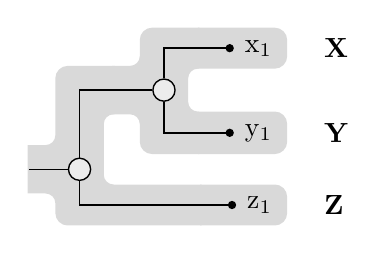
\begin{tikzpicture}
% background
\path[species background] (30.5,13.81) [rounded corners={4pt}] -- (10,13.81) -- (10,42.42) [sharp corners] -- (0,42.42) -- (0,58.92) [rounded corners={4pt}] -- (10,58.92) -- (10,70.4799) [sharp corners] -- (61.84,70.4799) -- (61.84,56.67) [rounded corners={4pt}] -- (26.5,56.67) -- (26.5,30.31) [sharp corners] -- (30.5,30.31) -- cycle;
\path[species background] (61.0,0) [rounded corners={4pt}] -- (40.5,0) -- (40.5,13.81) [sharp corners] -- (30.5,13.81) -- (30.5,30.31) [rounded corners={4pt}] -- (40.5,30.31) -- (40.5,44.67) [sharp corners] -- (61.0,44.67) -- (61.0,30.31) [rounded corners={4pt}] -- (57.0,30.31) -- (57.0,13.81) [sharp corners] -- (61.0,13.81) -- cycle;
\path[species background, rounded corners={4pt}] (61.0,0) -- (92.763,0) -- node[species label] {X} (92.763,13.81) -- (61.0,13.81);
\path[species background, rounded corners={4pt}] (61.0,30.31) -- (92.763,30.31) -- node[species label] {Y} (92.763,44.67) -- (61.0,44.67);
\path[species background, rounded corners={4pt}] (61.84,56.67) -- (92.763,56.67) -- node[species label] {Z} (92.763,70.4799) -- (61.84,70.4799);
% gene branches
\path[branch={reccolor0}] (14,50.67) -- (0,50.67);
\path[branch={reccolor0}] (30.5,22.06) -| (18.25,46.42) (18.25,54.92) |- (61.84,63.5749);
\path[branch={reccolor0}] (44.5,22.06) -- (30.5,22.06);
\path[branch={reccolor0}] (61.0,6.905) -| (48.75,17.81) (48.75,26.31) |- (61.0,37.49);
\path[branch={reccolor0}] (71.0,6.905) -- (61.0,6.905);
\path[branch={reccolor0}] (71.0,37.49) -- (61.0,37.49);
\path[branch={reccolor0}] (71.84,63.5749) -- (61.84,63.5749);
% gene transfers
% events
\node[speciation={reccolor0}] at (18.25,50.67) {};
\node[speciation={reccolor0}] at (48.75,22.06) {};
\node[extant gene={reccolor0}{x\textsubscript{1}}] at (72.5,6.905) {};
\node[extant gene={reccolor0}{y\textsubscript{1}}] at (72.5,37.49) {};
\node[extant gene={reccolor0}{z\textsubscript{1}}] at (73.34,63.5749) {};
\end{tikzpicture}
